\section{Discussion}

% Relation to previous work / Should rewrite this paragraph!
In our previous study, we demonstrated that oculomotor signals play a substantial role in the perception of translation, even in the absence of optic flow or any other visual stimulation \cite{clemens2015a}. Although the vestibular system provided the most significant contribution, oculomotor signals were shown to account for about 20\% of the overall percept. Because these experiments were performed with a single fixation depth, it was not clear whether the brain weighted the oculomotor signal in a depth-dependent manner when using it as a translation cue, or merely uses the signal as a rudimentary cue to self-motion. In the present study we tested between these two possibilities.

% Basic observations
We assessed translation perception during both body- and world-fixed fixation at two different fixation depths. Our results show that self-motion was underestimated when comparing far and near fixation trials in the world-fixed condition, which argues against a proper scaling of the eye movement signal. Fixation depth did not influence translation perception during body-fixed fixation (where eye movements are virtually absent).

% Model results
To quantify the relative depth-dependent scaling of eye movements for nearby and far away fixation targets, we fitted a straightforward linear model to the perceptual responses based on the oculomotor behavior across four conditions. While two participants show partial scaling, the other six participants did not show any sign of scaling. Thus, we conclude that while oculomotor signals provide a robust cue to translation perception, they are not properly scaled by fixation depth.


\subsection{Relation to other studies}

% Relation to Clemens, 2015
\begin{figure}
    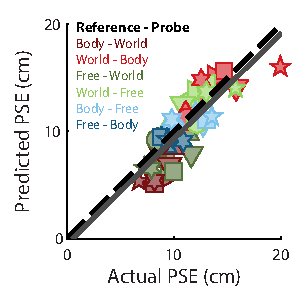
\includegraphics[width=0.5\textwidth]{src/paper4/p4_figure6.pdf}

    \caption{Predicted versus actual PSEs for Clemens \protect\citeyear{clemens2015a} using parameter $\alpha_{50}$ from the present paper. A data point (symbol) is shown for each participant (symbol shape) and condition (symbol color) pair, following the same color scheme as in \protect\figref{p3:fig2}: Body-world comparison; body reference, dark red; world reference, light red. World-free comparison; world reference, light green; free reference, dark green. Body-free comparison; body reference, dark blue; free reference, light blue.}
    \label{p4:fig6}
\end{figure}

In our previous experiment we compared translation perception with body-fixed versus world-fixed fixations at near depth (50 \si{\centi\metre}) only \cite{clemens2015a}. \figref{p4:fig6} shows how well our $\alpha_{50}$ parameter explains the data in our previous paper. The highly positive correlation between the actual PSEs in the previous study and those predicted using the model of the present paper ($\rho = 0.60$, $p = 0.06$) adds confidence to the parameter values presented here. The average difference between the values found here and those reported previously (see \tabref{p4:tab2}) is 12 \textpm 8 percent-points, which is relatively small given the indpendent measurements.

% Relation to the VOR
The function of the LVOR is to keep the eyes stable in the world during linear translation \cite{paige1989,busettini1994,paige1998}. Because it also needs to scale with fixation depth \cite{angelaki2004}, it is possible that both the LVOR and self-motion perception have the same underlying same signal. Because of the visual fixation point, visual following mechanisms may even augment the LVOR compensation. If the oculomotor signal generated by the LVOR is used for self-motion perception, one would expect that the LVOR compensation at 50 and 200cm closely relate to the corresponding oculomotor weights in the present study (see \figref{p4:fig5} and \tabref{p4:tab2}). To further explore this, we derived the LVOR gains for 50 and 200 \si{\centi\metre} from Paige et al. \citeyear{paige1989} and computed their expected depth ratio, $d_{200} / d_{50}$. This ratio, 1.87, is in between the ratio of the 6 participants who did not show any sign of scaling ($\frac{d_{200}}{d_{50}} = 1.07 \pm 0.16$) and the 2 participants that did show scaling ($\frac{d_{200}}{d_{50}} = 3.06 \pm 0.27$).


\subsection{Alternative explanations}

It is important to point out that while the vestibular signal and thus noise is constant for a given translation distance, the noise in the associated oculomotor estimate might not be, as the magnitude of the eye movement (i.e. signal-dependent noise) is modulated by fixation depth. If signal-dependent noise would play a role, nearby world-fixed fixations would cause larger eye movements with more noise compared to the far world-fixed fixations with smaller eye movements. The oculomotor based translation estimate would be weighted less for near versus far fixation, potentially explaining the partial compensation for fixation depth we have observed. In addition, the noise levels in the oculomotor estimate could also depend on fixation depth itself: the retinal displacement of a world stationary fixation point decreases with fixation depth, making it less informative about the amount of self-motion. The noise level in the oculomotor estimate would therefore be higher for far away compared to nearby fixation points. For world stationary targets, this would predict an underestimation of self-motion while fixating far away compared to nearby, which is in line with our observations. However, it also predicts a similar effect for body stationary targets. As no such effects between the near and far body stationary fixation targets have been observed, we consider it an unlikely alternative explanation.
 
Could the lack of scaling be explained by how participants perceive the distance of the fixation points? Because the difference between body- and world-fixed fixation points is reduced at far fixation distances, the lack of scaling could - in theory - be explained by participants incorrectly perceiving both the body- and world-fixed far fixation points as being body-fixed. We consider this an unlikely explanation, because the target displacement associated with a world-fixed target was between 0.3 and 8.5 degrees in our experiment, which is easily perceived. This adds confidence to our claim that eye movements influence self-motion perception, but with moderate to no scaling for fixation depth.


